\documentclass[11pt,letterpaper]{article}
\usepackage[margin=1in]{geometry}
\usepackage{graphicx}
\usepackage{hyperref}
\usepackage{listings}
\pagestyle{headings}
\author{Nina Stein}
\title{CompPhys 2 Exam}
\begin{document}
\maketitle

\section*{Problem 1}
 Alright, my python code for this is \begin{verbatim}
 wavepacket_midterm.py
 \end{verbatim}, I disobeyed you and made the potential barrier rather higher than it was originally so that you could see the effects more (they were slightly less obvious than I expected), as shown in the figures (I really wish I could just record the animation and play it back, rather than trying to show you in stills what happened). 
 \begin{figure}
 \includegraphics[width=0.9\linewidth]{movingbarrier.pdf}
 \end{figure}
\section*{Problem 2}
I did this in x and y before I got your response, sorry. Anyway, code is apparently not on this machine, will have to get back to you on that and the 3d figure, but the cutaway figure is shown, though I'm not entirely sure it matches the analyutics (I haven't done that calculation yet). In particular, I'm not sure if it should be going up inside the inner ring?
\begin{figure}
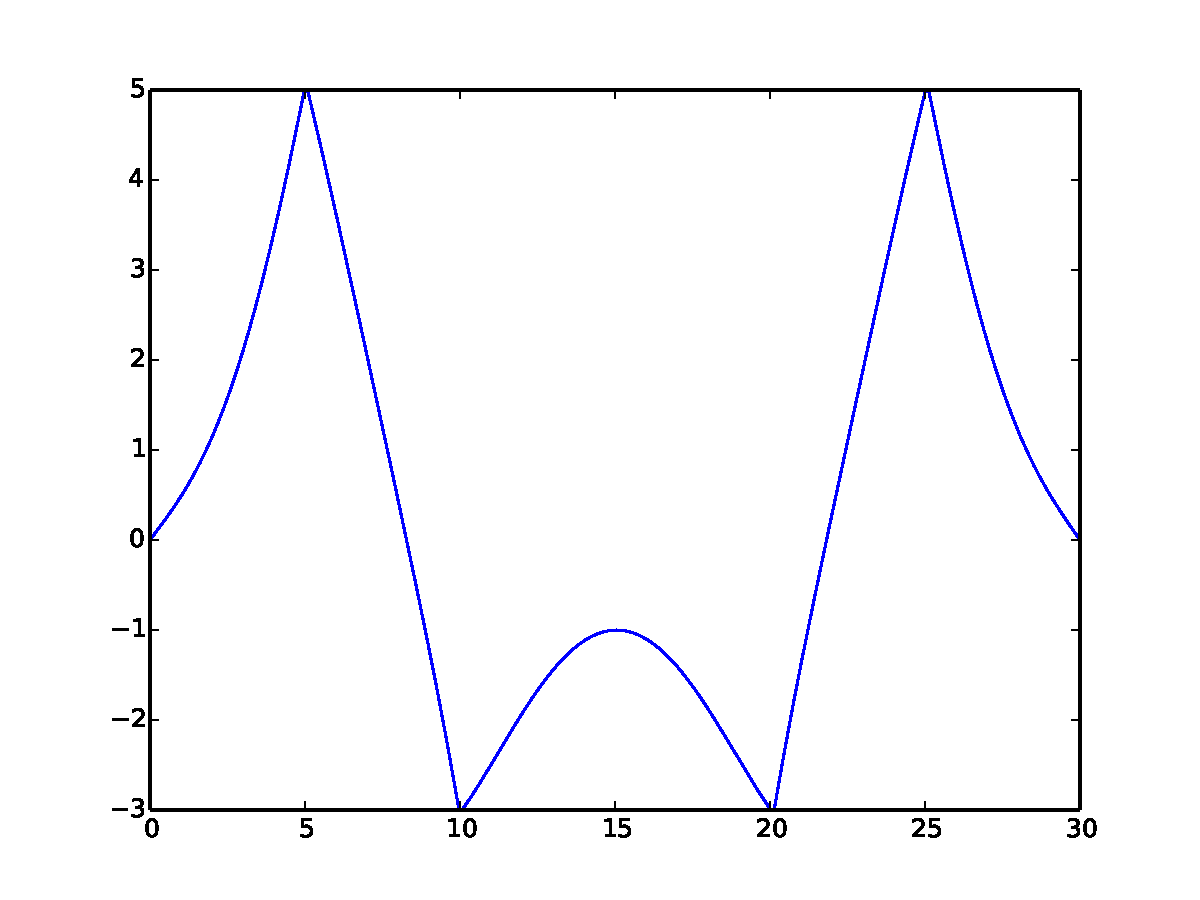
\includegraphics[width=0.9\linewidth]{cutaway.pdf}
\end{figure} 
\section*{Problem 3}
Alright, so my modified jupyter notebook is HW4P3.ipynb, and I have to start this with a caveat: I'm not actually sure I got this working right. I showed it to a friend of mine who does fluids, and he said it was definitely a much more sensible plot, but he wasn't entirely sure that it was entirely correct--it didn't look quite right to him. So. Not sure anymore. 

So, actually, I have two statements: If I didn't actually get it working, I blame the fact that it's a hugely complex and nonlinear set of equations, and the code is \textit{hilariously} unstable; I have a hard time really believing that I can reasonably or coherently determine whether or what I did wrong if the code is so unstable that simply changing the number of steps across the space spanned causes it to go catastrophically nuts. That said, my fluids friend has also suggested that a) the code is not designed for perturbations on the continuous flow, and might not have a correctly implemented curl term, and b) rigid/sharp edges are apparently infamous for causing problems in numerical flow calculations, so the very fact that my object is rectangular might be causing problems. 

The second statement is that what I did to go from crazy horseshoe crab explosion to something that looks about right is simply increase the size of the channel. Note that the barrier was proportionally increased, so that all that really changed was dx and dy, and I don't really know why that would help me, unless it's something about some sort of minimum step size to have the fluid calculations work (possibly related to renolds number?) or that a larger dx and dy means that the points adjacent to the boundary of my object are farther away from it, thus avoiding crazy madness, but there it is. 
Good lord this code is an unholy mess. 
\end{document}